\documentclass{jarticle}
\usepackage[dvipdfmx]{graphicx}
\usepackage{here}
\usepackage{listings,jlisting}


\lstset{
  basicstyle={\ttfamily},
  identifierstyle={\small},
  commentstyle={\smallitshape},
  keywordstyle={\small\bfseries},
  ndkeywordstyle={\small},
  stringstyle={\small\ttfamily},
  frame={tb},
  breaklines=true,
  columns=[l]{fullflexible},
  numbers=left,
  xrightmargin=0zw,
  xleftmargin=3zw,
  numberstyle={\scriptsize},
  stepnumber=1,
  numbersep=1zw,
  lineskip=-0.5ex
}

\title{{システム実験}\\実験14回レポート}
\author{6119019056 山口力也}
\date{2019/07/26日提出}

\begin{document}
\maketitle
\section{演習}

\subsection{目的}
カラーセンサによる色の表現方法やセンシング技術の理解を深めた.また,カラーセンサについて学んだ知識を統合的に応用した.特に,種々の測定環境で,効率よくカラーセンサのデータを測定する手法を習得した.

\subsection{演習8.2.1}
演習8.1.1に従い,カラーセンサの配線を行った.次に,演習8.1.2で使用したサンプルスケッチを用いて配線が正しく行われていることを確認した.

\subsection{演習8.2.2}
カラーパターンの白黒部分をセンサで計測し,シリアルモニタに表示された最小値と最大値を記録した.その後,Arduinoのサンプルスケッチのパラメータを手動で調整し,カラーセンサのキャリブレーションを行った. \\

\subsection{演習8.2.3}
手動キャリブレーションでは,カラーセンサのRGB値(最小・最大)を毎回記録し,プログラムに反映させなければならない.そこで,カラーパターンの白黒部分にセンサを5秒間かざせば,RGB値の最小・最大が決定できる様に改良した.

以下表\ref{table:enshu8-2-3}に,演習8.2.2と演習8.2.3の結果を示す. \\
手動キャリブレーションとオートキャリブレーションの結果の違いは小節\ref{subsec:kadai8-2-1}で考察する.

\begin{table}[H]
\caption{カラーパターンの各色のRGB値}
	\begin{center}
		\begin{tabular}{|c|c|c|c|c|c|c|}\hline 
			& \multicolumn{3}{c|}{手動キャリブレーション後}&\multicolumn{3}{c|}{自動キャリブレーション後} \\ \hline 
			& Red値 & Green値 & Blue値 & Red値 & Green値 & Blue値 \\ \hline 
		黒 & 3 & 4 & 3 & 13 & 12 & 0  \\ \hline
		白 & 219 & 306 & 225 & 469 & 342 & 384  \\ \hline 
		赤 & 136 & 39 & 23 & 232 & 45 & 52  \\ \hline
		緑 & 49 & 150 & 62& 93 & 252 & 113  \\ \hline
		青 & 53 & 97 & 145 & 44 & 75 & 182  \\ \hline
		シアン & 41 & 89 & 74 & 138 & 261 & 291  \\ \hline
		マゼンタ & 124 & 74 & 94 & 255 & 144 & 206  \\ \hline
		イエロー & 187 & 259 & 64 & 326 & 303 & 117  \\ \hline
		\end{tabular}
	\end{center}
\label{table:enshu8-2-3} 
\end{table}


\subsection{演習8.2.4}
この演習では,閾値法により色の識別を行なった.各色のRGB値を参考にしながら,色を正しく判定できるように閾値を決めた.
閾値には表\ref{table:enshu8-2-3}を参考にした.
考察は小節\ref{subsec:kadai8-2-3}で行なった.

\subsection{演習8.2.5}
試行錯誤による閾値の設定だけでは色を正しく認識するのは難しい.そこで,閾値を簡単に決める方法として機械学習アルゴリズムの一つであるk近傍法がある.特徴空間の中で最も近いラベルへ統計的に分類する手法である.これらを用いて色を認識した.
\begin{table}[H]
\caption{カラーパターンの各色に対するRGB値とその平均}
	\begin{center}
		\begin{tabular}{|c|c|c|c|c|c|c|c|c|c|c|c|c|}\hline 
		& \multicolumn{4}{c|}{Red値} & \multicolumn{4}{c|}{Green値} & \multicolumn{4}{c|}{Blue値} \\ \hline
			& 1 & 2 & 3 &平均& 1 & 2 & 3 &平均& 1 & 2 & 3 &平均 \\ \hline
		黒 & 0 & 6 & 4 & 3.3& 1 & 6 & 4 & 3.7& 0 & 5 & 3 & 2.7 \\ \hline
		白 &262&264&264&263.3&360&360&375&365&261&262&262&262.7 \\ \hline
		\end{tabular}
	\end{center}
\label{table:enshu8-2-5} 
\end{table}


\section{課題}

\subsection{課題8-2-1}\label{subsec:kadai8-2-1}
\ref{table:enshu8-2-3}の結果を用いて,手動キャリブレーションと自動キャリブレーションの違いを確認し,その結果が得られた理由を考察せよ.また,Processingの表示と一致するかどうかも報告せよ.

以下図\ref{fig:kadai8-2-1-m-b},図\ref{fig:kadai8-2-1-m-w},図\ref{fig:kadai8-2-1-a-w},図\ref{fig:kadai8-2-1-a-b}にそれぞれ手動キャリブレーションとオートキャリブレーション時の黒,白のセンシング時の結果を示す.

\begin{figure}[H]
\begin{center}
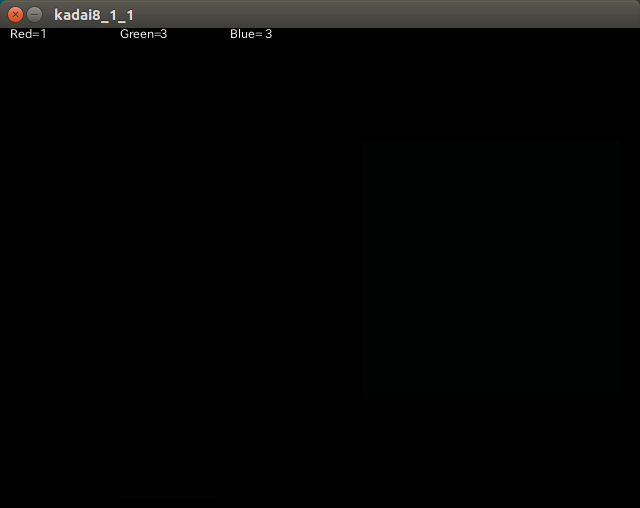
\includegraphics[width=7.0cm]{images/kadai8-1-1-manual-black.png}
\caption{手動キャリブレーション(黒)}
\label{fig:kadai8-2-1-m-b}
\end{center}
\end{figure}


\begin{figure}[H]
\begin{center}
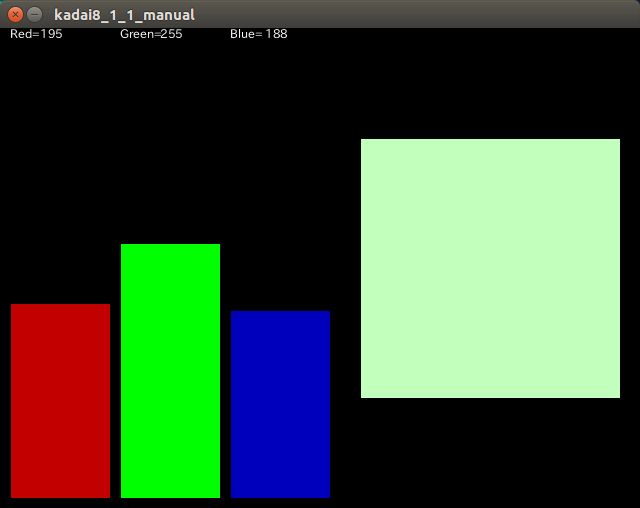
\includegraphics[width=7.0cm]{images/kadai8-1-1-manual-white.png}
\caption{手動キャリブレーション(白)}
\label{fig:kadai8-2-1-m-w}
\end{center}
\end{figure}

\begin{figure}[H]
\begin{center}
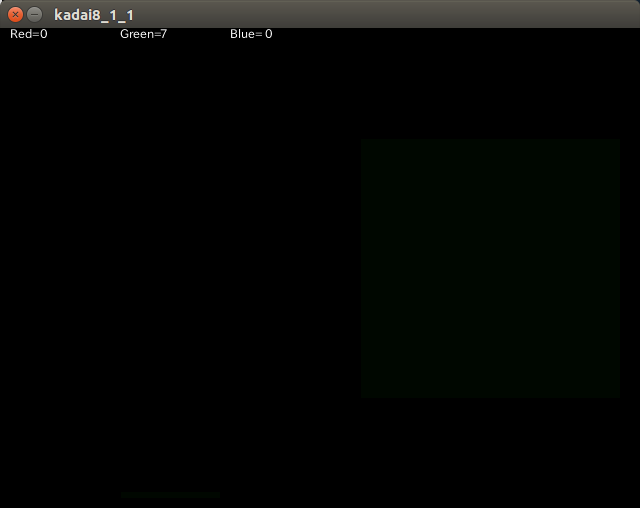
\includegraphics[width=7.0cm]{images/kadai8-1-1-auto-black-yoi.png}
\caption{自動キャリブレーション(黒)}
\label{fig:kadai8-2-1-a-b}
\end{center}
\end{figure}

\begin{figure}[H]
\begin{center}
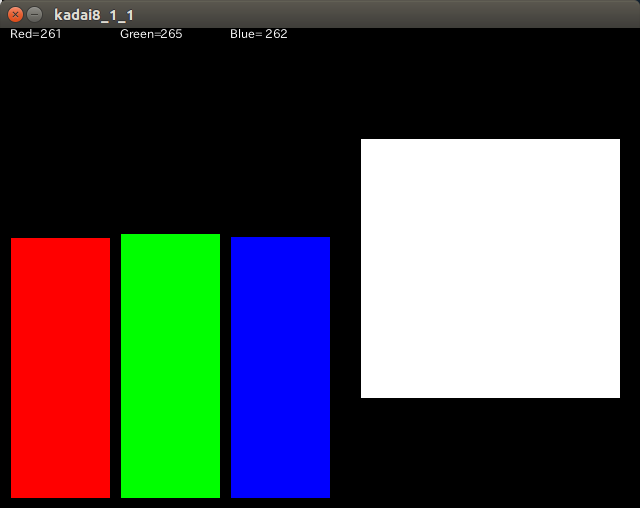
\includegraphics[width=7.0cm]{images/kadai8-1-1-auto-white-yoi.png}
\caption{自動キャリブレーション(白)}
\label{fig:kadai8-2-1-a-w}
\end{center}
\end{figure}

黒色の場合はどちらもうまくセンシングできているが,白色の場合は自動キャリブレーションはうまくセンシングできているが,手動キャリブレーションでは若干値が足りなく白色とは異なる色となった.これは手動キャリブレーション時に最大値,最小値の設定を誤っていたためと考えられる.map関数を用いて0$\sim$255の値に変換しているので最大値は合っていても最小値をうまく設定できていない場合,本来出るべき最大値がでない可能性がある. \\
手動キャリブレーション時,自分は10個ほどの値しか参考にしなかったため,自動キャリブレーションとでは比較する数が違うのも原因だと考えられる.

\subsection{課題8.2.2}\label{subsec:kadai8-2-2}

自動キャリブレーション時間の影響を調べるために,RGB値の最小,最大を決める時間を1秒と10秒でそれぞれ設定し,黒と白のRGB値を比較した.
以下表\ref{table:kadai8-2-2}に結果を示す.
\begin{table}[H]
\caption{カラーパターンの各色のRGB値}
	\begin{center}
		\begin{tabular}{|c|c|c|c|c|c|c|}\hline 
			& \multicolumn{3}{c|}{自動キャリブレーション(1s)}&\multicolumn{3}{c|}{自動キャリブレーション(10s)} \\ \hline 
			& Red値 & Green値 & Blue値& Red値 & Green値 & Blue値 \\ \hline
		黒 & 3 & 4 & 3 & 13 & 88 & 14 \\	 \hline
		白 & 73& 77& 14& 498& 506& 55\\ \hline 
		\end{tabular}
	\end{center}
\label{table:kadai8-2-2} 
\end{table}

キャリブレーションの時間が短いと最小値がうまくでなかった.が,逆に長すぎても最大値が大きく,また最小値も大きくなってしまった.そのため実際には適切な秒を選択するべきだと考えられる.
\subsection{課題8.2.3}\label{subsec:kadai8-2-3}
演習8.2.4の閾値法により,カラーパターンの赤,緑,青,シアン,マゼンタ,イエローの各色を正しく識別できる様にプログラムを変更せよ.

閾値には表\ref{table:enshu8-2-3}を参考にした.
以下ソースコード\ref{code:kadai8-2-3-a}にスケッチを示す.

\lstinputlisting[caption = 課題8.2.3(Arduino),label=code:kadai8-2-3-a]{./Arduino/kadai8-2-3/kadai8-2-3.ino}

黒や白などの大まかなものは大体認識できたが,シアンなどの中間色は誤って認識することが多かった.手動キャリブレーションでは値の決め方が難しいためだと考えられる.

\subsection{課題8.2.4}\label{subsec:kadai8-2-4}
演習8.2.5のk近傍法により,カラーパターンの赤,緑,青,シアン,マゼンタ,イエローの各色を正しく認識できる様にプログラムを変更せよ.
以下表\ref{table:kadai8-2-4}に各色に対するRGB値を示す.

\begin{table}[H]
\caption{カラーパターンの各色に対するRGB値とその平均}
	\begin{center}
		\begin{tabular}{|c|c|c|c|c|c|c|c|c|c|c|c|c|}\hline 
		& \multicolumn{4}{c|}{Red値} & \multicolumn{4}{c|}{Green値} & \multicolumn{4}{c|}{Blue値} \\ \hline
			& 1 & 2 & 3 &平均& 1 & 2 & 3 &平均& 1 & 2 & 3 &平均 \\ \hline
		黒 & 0 & 6 & 4 & 3.3& 1 & 6 & 4 & 3.7& 0 & 5 & 3 & 2.7 \\ \hline
		白 &262&264&264&263 &360&360&375&365&261&262&262&263 \\ \hline
		赤 &157&152&150& 153&75 &75 & 75& 75& 15& 15& 13&14 \\ \hline
		緑 & 44& 54 &47& 48 &170&182&176&176& 56& 45& 47&49 \\ \hline
		青 & 53& 56 &57& 55 & 75&80 &78 & 78&181&184&179&181 \\ \hline
 シアン & 41& 42& 45& 43 & 89& 95& 92& 92& 75& 80& 78& 78\\ \hline
 マゼンタ&124&128&134& 129& 76& 82& 77& 78&100&105&103& 103\\ \hline
 イエロー&190&186&193& 190&263&254&266&261& 70& 76& 88& 78\\ \hline
		\end{tabular}
	\end{center}
\label{table:kadai8-2-4} 
\end{table}

この表\ref{table:kadai8-2-4}を参考にk近傍法による色の識別を行なった.
作成したコードを以下ソースコード\ref{code:kadai8-2-4-a}に示す.

\lstinputlisting[caption = 課題8.2.4(Arduino),label=code:kadai8-2-4-a]{./Arduino/kadai8-2-4-new/kadai8-2-4-new.ino}

\subsection{課題8.2.5}
閾値法またはk近傍法どちらか一つを選び,Arduinoで識別した色をシリアル通信でProcessing側に送信し,センシングした色とともに識別結果を表示できる様にプログラムを変更せよ.

作成したコードを以下ソースコード\ref{code:kadai8-2-5-p}に示す.

\lstinputlisting[caption = 課題8.2.5(Processing),label=code:kadai8-2-5-p]{./Processing/kadai8_1_1/kadai8_1_1.pde}

また,プログラムの実行結果を以下図\ref{fig:kadai8-2-5}に示す.

\begin{figure}[H]
\begin{center}
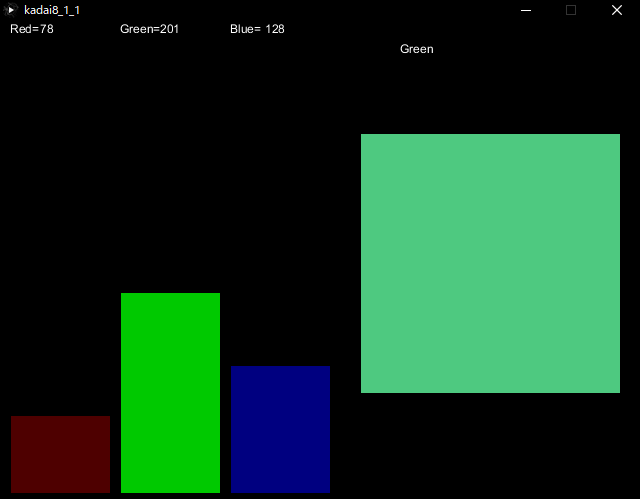
\includegraphics[width=7.0cm]{images/kadai8-2-5.png}
\caption{k近傍法による色の識別}
\label{fig:kadai8-2-5}
\end{center}
\end{figure}


\subsection{課題8.2.6}
課題8.2.5のプログラムを用いてカラーパターン境界域すべてについてセンシングを行い,Processingの表示により色を正しく識別できているか確認せよ.またその結果からどのような条件のとき色の誤認識が怒るのか,またどの様にすれば誤認識を改善できるか考察せよ.

以下図\ref{fig:kadai8-2-6}に結果の一例を示す.

\begin{figure}[H]
\begin{center}
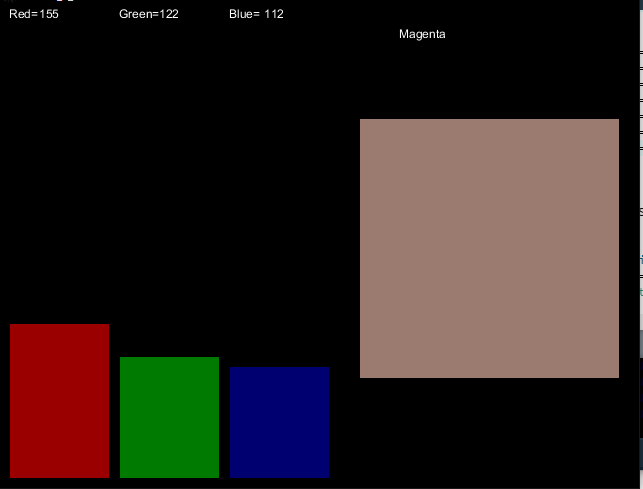
\includegraphics[width=7.0cm]{images/kadai8-2-6-new.png}
\caption{境界域での色の識別}
\label{fig:kadai8-2-6}
\end{center}
\end{figure}

図\ref{fig:kadai8-2-6}はシアンとマゼンタの境界域における実行結果である.\\
境界域では二つの色が混ざった様なRGB値が出てきて,今回はマゼンタと識別しているが他の境界域では全く異なる色と認識してしまう場合があった.改善するにはk近傍法の値を変えるか,あるいは最近傍法などの他の手法を用いるなどが考えられる.

\subsection{課題8.2.7}
課題8.2.5で作成したプログラムを用いて,手でセンサを素早く(またはゆっくり)カラーパターンの上で移動させた時,RGB値がどのように変化しているか確認せよ. また,カラーセンサが誤認識を起こす場合,その理由と改善策を考察せよ. \\

手を素早く移動させたとき,カラーセンサのRGB値が変化し,誤認識することが多かった.しかしながらRGB値の変化に統一性はなかったように思われる.
手をゆっくり移動させたとき,カラーセンサのRGB値は大きく増え,大体の場合「白」と認識することが多かった. \\
手を素早く移動させたときの状態を改善するには直近の何回かのセンシングの結果を保存しておきそれらの平均をとるなどをして急激な変化に耐えれるようにするなどが考えられる.
手をゆっくり移動させたときの状態を改善するには,RGB値が一定の値を超えたら識別しないようにすることが考えられる.手をゆっくり移動させた時,大体の場合白に識別され,またRGB値も普通の白の場合を大きく超えていた.それらを考慮してRGB値がある一定の値を超えたら識別を行わないなどをすると良いと考えられる.
\end{document}
